% 曲线元示意图
\begin{figure}[htbp]
  \centering
  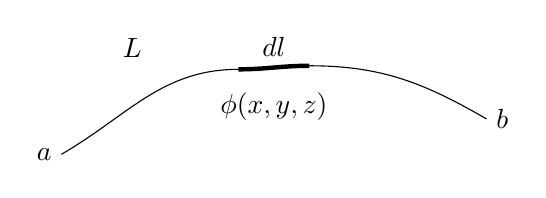
\begin{tikzpicture}[>=latex, scale=0.9]
    % 1. 定义关键坐标点
    % 起点
    \coordinate (start) at (0,0);
    % 粗线段的起点 (在中间位置)
    \coordinate (mid1) at (2.5, 1.2);
    % 粗线段的终点
    \coordinate (mid2) at (3.5, 1.25);
    % 终点
    \coordinate (end) at (6, 0.5);

    % 2. 绘制左半部分 (细线)
    % out=30, in=180 使得线条平滑地连向中间
    \draw (start) node[left] {$a$} 
          to[out=30, in=180] (mid1);

    % 3. 绘制中间部分 (加粗线段 dl)
    % ultra thick 加粗, midway 用于放置标签
    \draw[ultra thick] (mid1) 
          to[out=0, in=180] 
          node[midway, above] {$d l$} 
          node[midway, below=5pt] {$\phi(x,y,z)$} 
          (mid2);

    % 4. 绘制右半部分 (细线)
    \draw (mid2) 
          to[out=0, in=150] (end) 
          node[right] {$b$};

    % 5. 标注曲线名称 L
    \node at (1, 1.5) {$L$};

  \end{tikzpicture}
  \caption{}
  \label{fig:curve-element}
\end{figure}